\documentclass[hyperref={pdfpagelabels=false}]{beamer}
%\usepackage{href}
\usepackage{listings}
\usepackage[utf8]{inputenc}
\setbeamertemplate{section in toc}[sections numbered]
\setbeamertemplate{subsection in toc}[subsections numbered]
\newcommand{\pu}{PostgreSQL Überblick}
\newcommand{\rsql}{Rekursiver SQL Aufruf}
\newcommand{\tit}{Ausgewählte Systeme Postgres }
\newcommand{\parcht}{Postgres Architektur}
\newcommand{\mergebnisse}{Messergebnisse pgBench}
\newcommand{\storedproc}{Stored Procedure}
\newcommand{\pgbench}{pgBench}
\newcommand{\konzepte}{Konzepte für rekursive Anfragen}
\newcommand{\fazit}{Fazit}
\usepackage{pdfpages}
\usepackage{tikz}
\usepackage{fancybox}
\usepackage{geometry}
\usepackage{pdflscape}
\usepackage{pgfplots}
\usepackage{filecontents}
\pgfplotsset{compat=1.15}
%\usepackage{pgfplots}
\usepackage{pgfplotstable}
%\geometry{bottom=0.9in}
\usepackage{fancyhdr}
\setbeamertemplate{footline}[text line]{
	\parbox{\linewidth}{\vspace*{-20pt} \hyperlink{tableofcontent}{
\includegraphics[scale=0.03]{../images/rhein-sieg.jpg}} \hspace{1cm} \tit \hfill\insertshortauthor\hfill\insertpagenumber}}
\setbeamertemplate{navigation symbols}{}
\author{Jennifer Wittling, Rolf Kimmelmann, Jan Löffelsender}
\title{\tit}
\usepackage{lmodern}
\usepackage{amsmath}
\usepackage{graphicx}
\setcounter{tocdepth}{1}

\pgfplotsset{
discard if/.style 2 args={
    x filter/.code={
    \edef\tempa{\thisrow{#1}}
    \edef\tempb{#2}
    \ifx\tempa\tempb
    \def\pgfmathresult{inf}
    \fi
    }
},
discard if not/.style 2 args={
x filter/.code={
\edef\tempa{\thisrow{#1}}
\edef\tempb{#2}
\ifx\tempa\tempb
\else
\def\pgfmathresult{inf}
\fi
}
}}


\begin{document}
%\tikzstyle{node} = [text width=2em, text centered]
%\lstset{language=Python}
%\lstset{language=Python}

	\begin{frame}
	\titlepage
	\end{frame} 

	\begin{frame}
	\frametitle{Agenda}
	\hypertarget{tableofcontent}{}
	\tableofcontents
	\end{frame}

	\section{Statements}
	\begin{frame}
	\frametitle{Statements}
	\begin{itemize}
		\item innerJoinGenerator
		\item recursivesearch
		\item selectCascadingGenerator
		\item selectUnionGenerator
	\end{itemize}
	\end{frame}

	\section{pgbench}
	\begin{frame}
	\frametitle{pgbench}
    \begin{itemize}
			\item Kommandozeilentool zur Durchführung von Benchmark-Tests.
			\item Bei einem Benchmark-Test wird eine Menge von SQL-Statements beliebig oft wiederholt.
			\item Mit pgBench können mehrere Clients parallel gestartet werden.
			\item pgBench berechnet Anzahl der Transaktionen pro Sekunde sowie die Latenz.
	\end{itemize}	
	\end{frame}

	\section{Aufbau Benchmarking-Test}
	\begin{frame}
	\frametitle{Aufbau Benchmarking-Test}
		\scriptsize
		\begin{figure}[H]
			\tikzstyle{every node}=[draw=black,anchor=west]
			\usetikzlibrary{trees}
			\tikzstyle{file}=[draw=none]
			\begin{tikzpicture}[%
			grow via three points={one child at (0.5,-0.5) and
				two children at (0.5,-0.5) and (0.5,-1.0)},
			edge from parent path={(\tikzparentnode.south) |- (\tikzchildnode.west)}]
			\node {pgbench}
			child{ node[file]{pgbench.sh}}
			child { node {public\_epinions}
				child{ node[file]{pgbench.sh}}
			}
			child [missing] {}		
			child { node {public\_epinions\_with\_index}
				child{ node[file]{pgbench.sh}}
				child{node[file]{Select\_innerJoinGenerator\_1.sql}}
				child{node[file]{...}}
			}
			child [missing] {}
			child [missing] {}
			child [missing] {}	
			child { node {public\_epinions\_partitioned}
				child{ node[file]{pgbench.sh}}
				child{node[file]{Select\_innerJoinGenerator\_1.sql}}
				child{node[file]{...}}
			};
			\end{tikzpicture}
			%Reset Configuration
			\tikzstyle{every node}=[]
		\end{figure}
	\end{frame}


	\section{Laufzeit relation\_livejournal}
	\begin{frame}
	\frametitle{Laufzeit relation\_livejournal}
		\begin{figure}[H]
			\scriptsize
			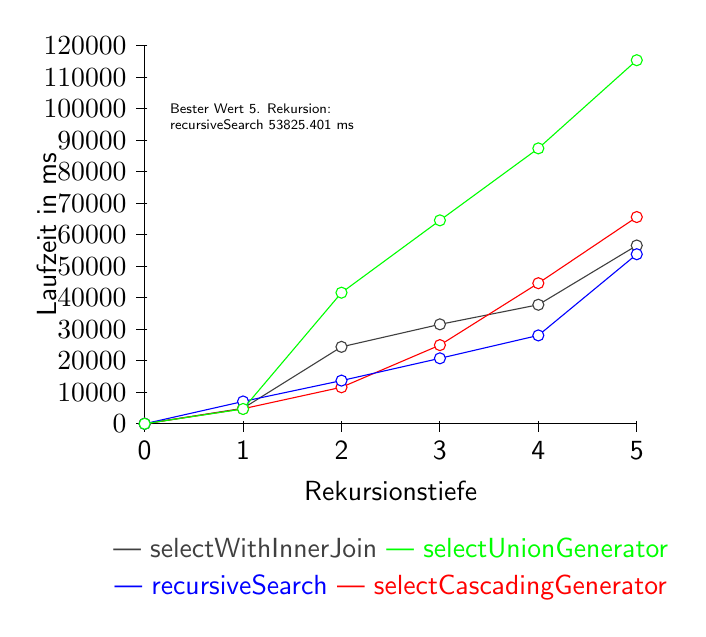
\begin{tikzpicture}[y=.2cm, x=1.25cm,font=\sffamily]
			%axis
			\draw (0,0) -- coordinate (x axis mid) (5,0);
			\draw (0,0) -- coordinate (y axis mid) (0,24);
			%ticks
			\foreach \x in {0,...,5}
			\draw (\x,1pt) -- (\x,-3pt)
			node[anchor=north] {\x};
			\foreach \y/\ytext in {
				0/0,	
				2/10000,
				4/20000,
				6/30000,
				8/40000,
				10/50000,
				12/60000,
				14/70000,
				16/80000,
				18/90000,
				20/100000,
				22/110000,
				24/120000
			}
			\draw (1pt,\y) -- (-3pt,\y) node[anchor=east] {$\ytext$};
			%labels      
			\node[below=0.6cm] at (x axis mid) {Rekursionstiefe};
			\node[rotate=90, above=1cm] at (y axis mid) {Laufzeit in ms};
			
			\draw[above=4cm, right=0.2cm ]
			node[draw=none]
			{
				\tiny Bester Wert 5. Rekursion:
				
				
			};
			\draw[above=3.8cm, right=0.2cm ]
			node[draw=none]
			{
				\tiny recursiveSearch 53825.401 ms
				
				
			};
			%plots
			\draw[darkgray] plot[mark=*, mark options={fill=white}] 
			coordinates{(0, 0)
				(1, 0.9819)%4909.862/5000)
				(2,	4.8836)%24417.787/5000)
				(3, 6.3127)%31563.339/5000)
				(4, 7.5570)%37785.200/5000)
				(5,	11.3202)%56601.185/5000)
			};
			\draw[red] plot[mark=*, mark options={fill=white}] 
			coordinates{(0, 0)
				(1, 4761.733/5000)
				(2,	11589.219/5000)
				(3, 4.9944)	%=24971/5000
				(4, 8.9252) %=44625,935÷5000
				(5,	13.1265944)%=65632,972÷5000
			};
			\draw[blue] plot[mark=*, mark options={fill=white}] 
			coordinates{(0, 0)
				(1, 1.4151)%7075.399/5000)
				(2,	2.7405)%13702.381/5000)
				(3, 4.1548)%20773.827/5000)
				(4, 5.6098)%28048.866/5000)
				(5,	10.7651)%53825.401/5000)
			};
			\draw[green] plot[mark=*, mark options={fill=white}] 
			coordinates{(0, 0)
				(1, 0.939)%4695.466/5000)
				(2,	8.323)%41616.216/5000)
				(3, 12.916)%64577.873/5000)
				(4, 17.487)%87434.075/5000)	
				(5,	23.086)%115432.071/5000)	
			};

			\draw[draw=none] (0,0) -- (5,0) 
			node[draw=none, midway, yshift=-4.5em]
			{
				\textcolor{darkgray}{--- selectWithInnerJoin}
				\textcolor{green}{--- selectUnionGenerator} 
				
			};
			\draw[draw=none] (0,-5) -- (5,0) 
			node[draw=none, midway, yshift=-4.5em]
			{
				\textcolor{blue}{--- recursiveSearch} 
				\textcolor{red}{--- selectCascadingGenerator}
			};
			\end{tikzpicture}
		\end{figure}
	\end{frame}
	\section{Laufzeit relation\_livejournal\_with\_index}
\begin{frame}
\frametitle{Laufzeit relation\_livejournal\_with\_index}
\begin{figure}[H]
	\scriptsize
	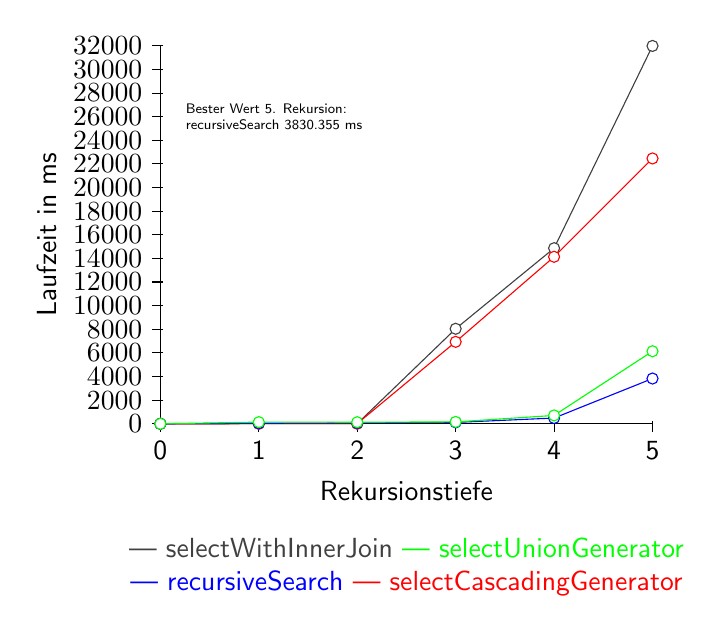
\begin{tikzpicture}[y=.3cm, x=1.25cm,font=\sffamily]
	%axis
	\draw (0,0) -- coordinate (x axis mid) (5,0);
	\draw (0,0) -- coordinate (y axis mid) (0,16);
	%ticks
	\foreach \x in {0,...,5}
	\draw (\x,1pt) -- (\x,-3pt)
	node[anchor=north] {\x};
	\foreach \y/\ytext in {
		0/0,
		1/2000,
		2/4000,
		3/6000,
		4/8000,
		5/10000,
		6/12000,
		7/14000,
		8/16000,
		9/18000,
		10/20000,
		11/22000,
		12/24000,
		13/26000,
		14/28000,
		15/30000,
		16/32000,
	}
	\draw (1pt,\y) -- (-3pt,\y) node[anchor=east] {$\ytext$};
	%labels      
	\node[below=0.6cm] at (x axis mid) {Rekursionstiefe};
	\node[rotate=90, above=1.2cm] at (y axis mid) {Laufzeit in ms};
	
	\draw[above=4cm, right=0.2cm ]
	node[draw=none]
	{
		\tiny Bester Wert 5. Rekursion:
		
		
	};
	\draw[above=3.8cm, right=0.2cm ]
	node[draw=none]
	{
		\tiny recursiveSearch 3830.355 ms
		
		
	};
	
	%plots
	
	\draw[darkgray] plot[mark=*, mark options={fill=white}] 
	coordinates{(0, 0)
		(1, 9.165/2000)
		(2,	11.862/2000)
		(3, 8042.794/2000)
		(4, 14865.814/2000)
		(5,	 15.995)%31990.436/2000)
	};	
	\draw[red] plot[mark=*, mark options={fill=white}] 
	coordinates{(0, 0)
		(1, 0.004)%8.672/2000
		(2,	15.240/2000)
		(3, 6936.935/2000)
		(4, 14137.544/2000)%
		(5,	11.232)%22464.363/2000	
	};
	\draw[blue] plot[mark=*, mark options={fill=white}] 
	coordinates{(0, 0)
		(1, 42.010/2000)
		(2,	69.129/2000)
		(3, 114.466/2000)
		(4, 484.914/2000)
		(5,	3830.355/2000)
	};
	\draw[green] plot[mark=*, mark options={fill=white}] 
	coordinates{(0, 0)
		(1, 139.294/2000)
		(2,	131.623/2000)
		(3, 157.707/2000)
		(4, 705.293/2000)
		(5, 6140.824/2000)
	};
	\draw[draw=none] (0,0) -- (5,0) 
	node[draw=none, midway, yshift=-4.5em]
	{
		\textcolor{darkgray}{--- selectWithInnerJoin}
		\textcolor{green}{--- selectUnionGenerator} 
		
	};
	\draw[draw=none] (0,-3) -- (5,0) 
	node[draw=none, midway, yshift=-4.5em]
	{
		\textcolor{blue}{--- recursiveSearch} 
		\textcolor{red}{--- selectCascadingGenerator}
	};
	
	\end{tikzpicture}
\end{figure}
\end{frame}
\section{Laufzeit relation\_livejournal\_partitioned}
\begin{frame}
\frametitle{Laufzeit relation\_livejournal\_partitioned}
		\begin{figure}[H]
	\scriptsize
	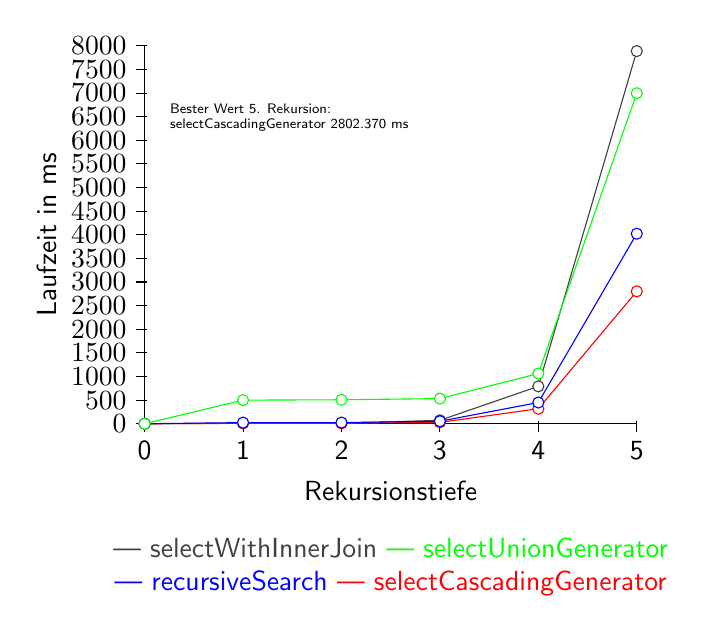
\begin{tikzpicture}[y=.3cm, x=1.25cm,font=\sffamily]
	%axis
	\draw (0,0) -- coordinate (x axis mid) (5,0);
	\draw (0,0) -- coordinate (y axis mid) (0,16);
	%ticks
	\foreach \x in {0,...,5}
	\draw (\x,1pt) -- (\x,-3pt)
	node[anchor=north] {\x};
	\foreach \y/\ytext in {
		0/0,
		1/500,
		2/1000,
		3/1500,
		4/2000,
		5/2500,
		6/3000,
		7/3500,
		8/4000,
		9/4500,
		10/5000,
		11/5500,
		12/6000,
		13/6500,
		14/7000,
		15/7500,
		16/8000
	}
	\draw (1pt,\y) -- (-3pt,\y) node[anchor=east] {$\ytext$};
	%labels      
	\node[below=0.6cm] at (x axis mid) {Rekursionstiefe};
	\node[rotate=90, above=1cm] at (y axis mid) {Laufzeit in ms};
	%plots
	\draw[above=4cm, right=0.2cm ]
	node[draw=none]
	{
		\tiny Bester Wert 5. Rekursion:
		
		
	};
	\draw[above=3.8cm, right=0.2cm ]
	node[draw=none]
	{
		\tiny selectCascadingGenerator 2802.370 ms
		
		
	};
	%InnerJoin
	\draw[darkgray] plot[mark=*, mark options={fill=white}] 
	coordinates{(0, 0)
		(1, 11.849/500)
		(2,	13.616/500)
		(3, 72.842/500)
		(4, 792.107/500)
		(5,	7888.135/500)
	};
	%SelectGenerator
	\draw[red] plot[mark=*, mark options={fill=white}] 
	coordinates{(0, 0)
		(1, 0.018)%8.945/500
		(2,	9.875/500)
		(3, 29.855/500)
		(4, 317.921/500)%
		(5,	2802.370/500)	
	};
	%RecursiveSearch
	\draw[blue] plot[mark=*, mark options={fill=white}] 
	coordinates{(0, 0)
		(1, 24.721/500)
		(2,	25.354/500)
		(3, 53.544/500)
		(4, 449.968/500)
		(5,	4022.937/500)
	};
	%SelectWithUnion
	\draw[green] plot[mark=*, mark options={fill=white}] 
	coordinates{(0, 0)
		(1, 500.063/500)
		(2,	507.950/500)
		(3, 532.557/500)
		(4, 1062.957/500)
		(5, 6995.607/500)
	};
	\draw[draw=none] (0,0) -- (5,0) 
	node[draw=none, midway, yshift=-4.5em]
	{
		\textcolor{darkgray}{--- selectWithInnerJoin}
		\textcolor{green}{--- selectUnionGenerator} 
		
	};
	\draw[draw=none] (0,-3) -- (5,0) 
	node[draw=none, midway, yshift=-4.5em]
	{
		\textcolor{blue}{--- recursiveSearch} 
		\textcolor{red}{--- selectCascadingGenerator}
	};
	
	\end{tikzpicture}
\end{figure}
\end{frame}

\section{Laufzeit relation\_epinions}
 \begin{frame}
 \frametitle{Laufzeit relation\_epinions}
 	\scriptsize
 	\begin{figure}[H]
 		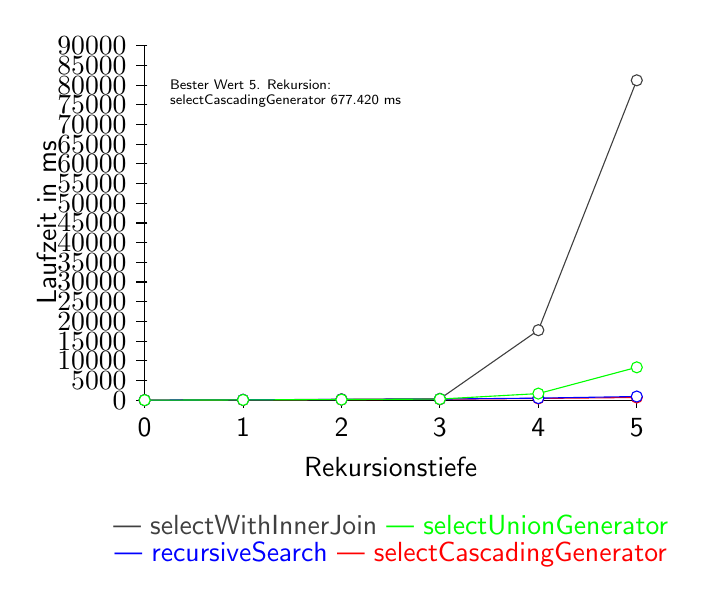
\begin{tikzpicture}[y=.25cm, x=1.25cm,font=\sffamily]
 		%axis
 		\draw (0,0) -- coordinate (x axis mid) (5,0);
 		\draw (0,0) -- coordinate (y axis mid) (0,18);
 		%ticks
 		\foreach \x in {0,...,5}
 		\draw (\x,1pt) -- (\x,-3pt)
 		node[anchor=north] {\x};
 		\foreach \y/\ytext in {
 			0/0,
 			1/5000,
 			2/10000,
 			3/15000,
 			4/20000,
 			5/25000,
 			6/30000,
 			7/35000,
 			8/40000,
 			9/45000,
 			10/50000,
 			11/55000,
 			12/60000,
 			13/65000,
 			14/70000,
 			15/75000,
 			16/80000,
 			17/85000,
 			18/90000
 		}
 		\draw (1pt,\y) -- (-3pt,\y) node[anchor=east] {$\ytext$}; 
 		%labels      
 		\node[below=0.6cm] at (x axis mid) {Rekursionstiefe};
 		\node[rotate=90, above=1cm] at (y axis mid) {Laufzeit in ms};
 		\draw[above=4cm, right=0.2cm ]
 		node[draw=none]
 		{
 			\tiny Bester Wert 5. Rekursion:
 			
 			
 		};
 		\draw[above=3.8cm, right=0.2cm ]
 		node[draw=none]
 		{
 			\tiny selectCascadingGenerator 677.420 ms
 			
 			
 		};
 		%plots
 		\draw[darkgray] plot[ mark=*, mark options={fill=white}] 
 		coordinates{(0, 0)
 			(1, 61.065/5000)
 			(2,231.850/5000)
 			(3,333.011/5000)
 			(4,3.5545)%17772.456/5000)
 			(5,16.2483)%81241.284/5000
 		};
 		
 		\draw[red] plot[ mark=*, mark options={fill=white}] 
 		coordinates{(0, 0)
 			(1, 63.636/5000)
 			(2,139.225/5000)
 			(3,229.997/5000)
 			(4,432.297/5000)
 			(5,677.420/5000)
 		};
 		\draw[blue] plot[ mark=*, mark options={fill=white}] 
 		coordinates{(0, 0)
 			(1, 89.858/5000)
 			(2,168.822/5000)
 			(3,273.452/5000)
 			(4,513.038/5000)
 			(5,921.228/5000)
 		};
 		\draw[green] plot[ mark=*, mark options={fill=white}] 
 		coordinates{(0, 0)
 			(1, 59.275/5000)
 			(2,143.367/5000)
 			(3,277.766/5000)
 			(4,1664.168/5000)
 			(5,8335.513/5000)
 		};
 		\draw[draw=none] (0,0) -- (5,0) 
 		node[draw=none, midway, yshift=-4.5em]
 		{
 			\textcolor{darkgray}{--- selectWithInnerJoin}
 			\textcolor{green}{--- selectUnionGenerator} 
 			
 		};
 		\draw[draw=none] (0,-3) -- (5,0) 
 		node[draw=none, midway, yshift=-4.5em]
 		{
 			\textcolor{blue}{--- recursiveSearch} 
 			\textcolor{red}{--- selectCascadingGenerator}
 		};
 		\end{tikzpicture}
 	\end{figure}
 \end{frame}

\section{Laufzeit relation\_epinions\_with\_index}
\begin{frame}
\frametitle{Laufzeit relation\_epinions\_with\_index}
	 	\scriptsize
\begin{figure}[H]
	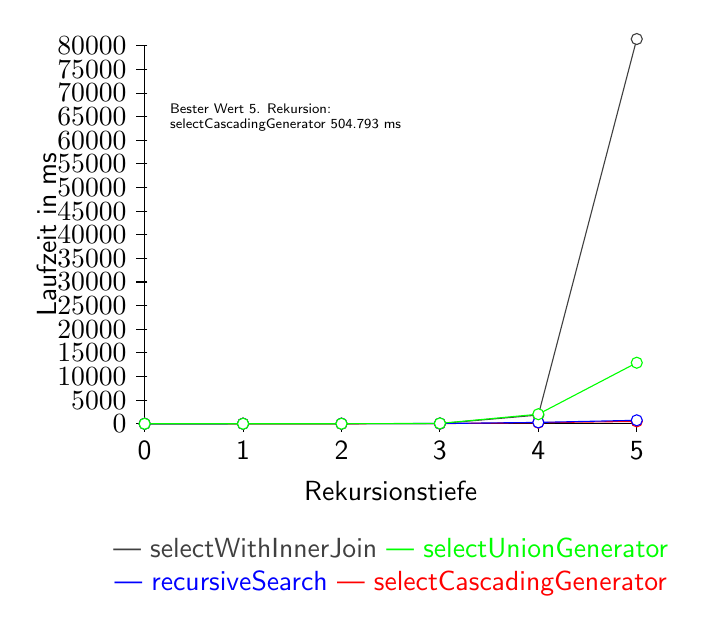
\begin{tikzpicture}[y=.3cm, x=1.25cm,font=\sffamily]
	%axis
	\draw (0,0) -- coordinate (x axis mid) (5,0);
	\draw (0,0) -- coordinate (y axis mid) (0,16);
	%ticks
	\foreach \x in {0,...,5}
	\draw (\x,1pt) -- (\x,-3pt)
	node[anchor=north] {\x};
	\foreach \y/\ytext in {
		0/0,
		1/5000,
		2/10000,
		3/15000,
		4/20000,
		5/25000,
		6/30000,
		7/35000,
		8/40000,
		9/45000,
		10/50000,
		11/55000,
		12/60000,
		13/65000,
		14/70000,
		15/75000,
		16/80000
	}
	\draw (1pt,\y) -- (-3pt,\y) node[anchor=east] {$\ytext$}; 
	%labels      
	\node[below=0.6cm] at (x axis mid) {Rekursionstiefe};
	\node[rotate=90, above=1cm] at (y axis mid) {Laufzeit in ms};
	\draw[above=4cm, right=0.2cm ]
	node[draw=none]
	{
		\tiny Bester Wert 5. Rekursion:
		
		
	};
	\draw[above=3.8cm, right=0.2cm ]
	node[draw=none]
	{
		\tiny selectCascadingGenerator 504.793 ms
		
		
	};
	%plots
	\draw[darkgray] plot[ mark=*, mark options={fill=white}] 
	coordinates{(0, 0)
		(1, 10.596/5000)
		(2, 10.739/5000)
		(3, 41.171/5000)
		(4, 0.3696)%1898.726/5000
		(5, 16.2872)%81436.561/5000
	};
	
	\draw[red] plot[ mark=*, mark options={fill=white}] 
	coordinates{(0, 0)
		(1, 8.231/5000)
		(2, 9.290/5000)
		(3, 36.244/5000)
		(4, 235.146/5000)
		(5, 504.793/5000)
	};
	\draw[blue] plot[ mark=*, mark options={fill=white}] 
	coordinates{(0, 0)
		(1, 18.999/5000)
		(2, 23.549/5000)
		(3, 54.953/5000)
		(4, 287.319/5000)
		(5, 737.300/5000)
	};
	\draw[green] plot[ mark=*, mark options={fill=white}] 
	coordinates{(0, 0)
		(1, 8.855/5000)
		(2, 10.304/5000)
		(3, 78.303/5000)
		(4, 2024.069/5000)
		(5, 12920.747/5000)
	};
	\draw[draw=none] (0,0) -- (5,0) 
	node[draw=none, midway, yshift=-4.5em]
	{
		\textcolor{darkgray}{--- selectWithInnerJoin}
		\textcolor{green}{--- selectUnionGenerator} 
		
	};
	\draw[draw=none] (0,-3) -- (5,0) 
	node[draw=none, midway, yshift=-4.5em]
	{
		\textcolor{blue}{--- recursiveSearch} 
		\textcolor{red}{--- selectCascadingGenerator}
	};
	\end{tikzpicture}
\end{figure}

	
\end{frame}

\section{Laufzeit relation\_epinions\_partitioned}
\begin{frame}
\frametitle{Laufzeit relation\_epinions\_partitioned}
	 	\scriptsize
\begin{figure}[H]
	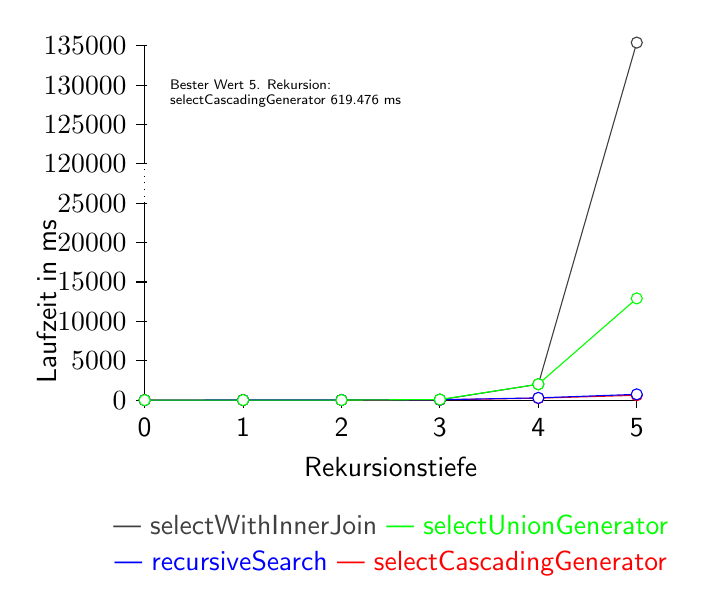
\begin{tikzpicture}[y=.5cm, x=1.25cm,font=\sffamily]
	%axis
	\draw (0,0) -- coordinate (x axis mid) (5,0);
	\draw (0,0) -- coordinate (y axis mid) (0,5);
	\draw[dotted] (0,5) -- (0,6);
	\draw (0,6) -- (0,9);
	%ticks
	\foreach \x in {0,...,5}
	\draw (\x,1pt) -- (\x,-3pt)
	node[anchor=north] {\x};
	\foreach \y/\ytext in {
		0/0,
		1/5000,
		2/10000,
		3/15000,
		4/20000,
		5/25000,
		6/120000,
		7/125000,
		8/130000,
		9/135000
	}
	\draw (1pt,\y) -- (-3pt,\y) node[anchor=east] {$\ytext$};
	%labels      
	\node[below=0.6cm] at (x axis mid) {Rekursionstiefe};
	\node[rotate=90, above=1cm] at (y axis mid) {Laufzeit in ms};
	%plots
	\draw[above=4cm, right=0.2cm ]
	node[draw=none]
	{
		\tiny Bester Wert 5. Rekursion:
		
		
	};
	\draw[above=3.8cm, right=0.2cm ]
	node[draw=none]
	{
		\tiny selectCascadingGenerator 619.476 ms
		
		
	};
	\draw[darkgray] plot[ mark=*, mark options={fill=white}] 
	coordinates{(0, 0)
		(1, 0.002)%8.846/5000)
		(2, 0.002)%9.924/5000)
		(3, 43.439/5000)
		(4, 2021.028/5000)
		(5, 9.082)%136242.608/15000)
	};
	
	\draw[red] plot[ mark=*, mark options={fill=white}] 
		coordinates{(0, 0)
		(1, 0.002)%8.730/5000)
		(2, 0.002)%9.787/5000)
		(3, 38.955/5000)
		(4, 253.813/5000)
		(5, 619.476/5000)
	};
	\draw[blue] plot[ mark=*, mark options={fill=white}] 
	coordinates{(0, 0)
		(1, 18.999/5000)
		(2, 23.549/5000)
		(3, 54.953/5000)
		(4, 287.319/5000)
		(5, 737.300/5000)
	};
	\draw[green] plot[ mark=*, mark options={fill=white}] 
	coordinates{(0, 0)
		(1, 8.855/5000)
		(2, 10.304/5000)
		(3, 78.303/5000)
		(4,2024.069/5000)
		(5,12920.747/5000)
	};
	\draw[draw=none] (0,0) -- (5,0) 
	node[draw=none, midway, yshift=-4.5em]
	{
		\textcolor{darkgray}{--- selectWithInnerJoin}
		\textcolor{green}{--- selectUnionGenerator} 
		
	};
	\draw[draw=none] (0,-2) -- (5,0) 
	node[draw=none, midway, yshift=-4.5em]
	{
		\textcolor{blue}{--- recursiveSearch} 
		\textcolor{red}{--- selectCascadingGenerator}
	};
	\end{tikzpicture}
\end{figure}
\end{frame}

\section{Fazit}
\begin{frame}
\frametitle{Fazit}
	\begin{itemize}
		\item Installation/Administration von PostgreSQL einfach und gut dokumentiert
		\item Fünfte Rekursionsstufe wird für alle Datensätze erreicht
		\item InnerJoin-Statements in der fünften Rekursionsstufe in fast allen Fällen am schlechtesten
		\item Latenz steigt stark bei hoher Anzahl an Input
		\item Indices und Partionierte Tabellen helfen vor allem bei großen Tabellen
\end{itemize}	
\end{frame}

\end{document}



